\documentclass[UKenglish]{beamer}


\usetheme{MathDept}
\usepackage{presentation}
\usepackage{style}


\day = 8
\month = 11
\year = 2017

\title{Join of hexagons and {Calabi--Yau} threefolds}
\subtitle{Public defence}
\author{Fredrik Meyer}


\begin{document}

\section{Outline}
\begin{frame}
\frametitle{Outline of the thesis}

\begin{itemize}
	\item Unsuccessful attempt to find new hyper-Kähler varieties.
	\item The topology of $C(\dP6)$.
	\item New Calabi--Yau varieties and potential mirror partners.
\end{itemize}

\end{frame}

\section{Stanley--Reisner schemes}
\begin{frame}
\frametitle{Stanley--Reisner schemes}


\begin{itemize}
	\item Given a simplicial complex $\mathcal F$, we get a Stanley--Reisner scheme $\P(\mathcal F)$.
	\item Is a union of projective spaces $\P^{\dim f}$, where $f$ is a face of $\mathcal F$.
\end{itemize}


\begin{example}

From a simplicial complex to a union of $\P^1$'s.

\begin{center}
\tikzstyle{ball} = [circle,shading=ball, ball color=uiored!80!white,
    minimum size=0.01cm]
\begin{tikzpicture}
\coordinate (A) at (2.5,-1.2);
\coordinate (B) at (4.1, -1.2);
\coordinate (C) at (5, 0);
\coordinate (D) at (4.1, 1.2);
\coordinate (E) at (2.5, 1.2);
\coordinate (F) at (1.6, 0);

\draw (A) -- (B) -- (C) -- (D) -- (E) -- (F) -- cycle;

\node[style=ball, scale=0.5] at (A) {};
\node[style=ball, scale=0.5] at (B) {};
\node[style=ball, scale=0.5] at (C) {};
\node[style=ball, scale=0.5] at (D) {};
\node[style=ball, scale=0.5] at (E) {};
\node[style=ball, scale=0.5] at (F) {};

\draw (6.8,-1) -- (9.2,-1); % E_1
\draw (8.4,-1.2) -- (9.7,0.3); % L_12
\draw (7.6,-1.2) -- (6.3,0.3); % L_13
\draw (8.4,1.2) -- (9.7,-0.3);
\draw (7.6,1.2) -- (6.3,-0.3);
\draw (6.8,1) -- (9.2, 1); % L_23
\end{tikzpicture}
\end{center}

The ideal is generated by $x_ix_{i+2}=x_ix_{i+3}=0$ ($i=0,\ldots,5$).

\end{example}
\end{frame}


\begin{frame}
\frametitle{Stanley--Reisner schemes}

\begin{itemize}
	\item \emph{Join} of two subschemes $X$ and $Y$: the (closure of) the union of all lines between $X$ and $Y$.
	\item \emph{Join} of two Stanley--Reisner schemes $\P(\mathcal F)$ and $\P(\mathcal G)$ is $\P(\mathcal F \ast \mathcal G)$, where the faces of $\mathcal F  \ast \mathcal G$ are $f \sqcup g$ for $f \in \mathcal F$, $g \in \mathcal G$.
\end{itemize}

\pause

Smoothings of Stanley--Reisner schemes: \pause

\begin{itemize}
	\item Given a basis for $T^1(S_{\P(\mathcal K)}/k,S_{\P(\mathcal K)})_0$, we can try to find a smoothing of $X_0 = \P(\mathcal K)$.
	\item A smoothing $X$ of $X_0$ will have many of the same properties:
		\begin{itemize}
			\item The same Hilbert polynomial.
			\item By semicontinuity, if $X_0$ is a sphere, $X$ will be Calabi--Yau. %% which we define now
		\end{itemize}
\end{itemize}


\end{frame}

\section{Calabi--Yau varieties}
\begin{frame}
\frametitle{\CY varieties}

\begin{definition}%[\CY variety]
    A \alert{\CY variety} is an irreducible, smooth, projective scheme $X/\C$ of dimension~$3$ satisfying:
    \begin{itemize}
      \item
      $H^0(X, \OO_X) = H^3(X, \OO_X) = \C$ and $H^1(X, \OO_X) = H^2(X, \OO_X) = 0$.

      \item
      The canonical sheaf is trivial: $\omega_X \simeq \OO_X$. 
    \end{itemize}
\end{definition}

\pause

\unskip
\begin{columns}[onlytextwidth]
    \begin{column}{0.6\textwidth}
        \begin{itemize}
          \item
          Easiest invariants are the \alert{Euler characteristic} and the \alert{Hodge numbers}, $h^{ij} = h^j\left(X, \Omega_{X/\C}^i\right)\mkern-2mu$.
          \pause

            \item
            We always have $\chi = 2(h^{11} - h^{12})$. 
        \end{itemize}
    \end{column}
\end{columns}

\only<2-3>
{
    \begin{textblock}{0.4}(0.58, 0.58)
        \[
            \arraycolsep = 1pt
            \def\arraystretch{0.5}
            \begin{array}[c]{ccccccc}
                &&& h^{00}                               \\  
                &&  h^{01} && h^{10}                     \\
                &   h^{02} && h^{11} && h^{20}           \\
                    h^{03} && h^{12} && h^{21} && h^{30} \\
                &   h^{13} && h^{22} && h^{31}           \\
                &&  h^{23} && h^{32}                     \\
                &&& h^{33} 
            \end{array}
        \]  
    \end{textblock}
}

\only<4->
{
    \begin{textblock}{0.4}(0.58, 0.58)
        \[
            \arraycolsep = 1pt%.5pt
            \def\arraystretch{0.5}%7}
            \begin{array}[c]{ccccccc}
                \phantom{h^03}  & \phantom{h^{02}} & \phantom{20} & 1 \\
                &&  0 && 0      & \phantom{h^30}                      \\
                &   0 && h^{11} && 0                                  \\
                    1 && h^{12} && h^{12} && 1                        \\
                &   0 && h^{11} && 0                                  \\
                &&  0 && 0 \vphantom{h^{32}}                          \\
                &&& 1 &&   \vphantom{h^{33}}
            \end{array}
        \]
    \end{textblock}
}
\end{frame}

\begin{frame}
\frametitle{Hodge numbers heuristic}

The quintic $X = V(f) \subset \P^4$ is the canonical example of a \CY. It has Hodge numbers $h^{11}=1$ and $h^{12}=101$.

\pause

\begin{proof}[Heuristic]
    The number $h^{12}$ is the dimension of the ``space of parameters'' of $X$. The following heuristic will give us the correct Hodge number:
    \pause
    \begin{itemize}[<+->]
      \item
      The space of degree $5$ polynomials $H^0\big(\P^4, \OO_{\P^4}(5)\big)$ in $\P^4$ is $\binom{4 + 5}{4} = \binom{9}{4} = 126$-dimensional. Hence $\P\big(H^0\big(\P^4, \OO_{\P^4}(5)\big)\big) = \P^{125}\mkern-4mu$.

      \item
      This is not unique, but we can act by $\PGL(5)$ to identify isomorphic quintics. We have $\dim \PGL(5)=25-1=24$.

      \item
      In total: $125 - 24 = 101$, which is $h^{12}(X)$.
      \qedhere
    \end{itemize}
\end{proof}

\end{frame}
% This frame contains a lot of text
% with no highlighting or overlay effects

\begin{frame}
\frametitle{Hodge numbers}

The quintic $X = V(f) \subset \P^4$ is the canonical example of a \CY. It has Hodge numbers $h^{11}=1$ and $h^{12}=101$.

\begin{remark}[Heuristic]
    The number $h^{12}$ is the dimension of the ``space of parameters'' of $X$. The following heuristic will give us the correct Hodge number:
    \begin{itemize}
	    \item
	    The space of degree $5$ polynomials $H^0\big(\P^4, \OO_{\P^4}(5)\big)$ in $\P^4$ is $\binom{4 + 5}{5} = \binom{9}{4} = 126$-dimensional. Hence $\P\big(H^0\big(\P^4, \OO_{\P^4}(5)\big)\big) = \P^{125}$.

	    \item
	    This is not unique, but we can act by $\PGL(5)$ to identify isomorphic quintics. We have $\dim \PGL(5)=25-1=24$.

	    \item
	    In total: $125 - 24 = 101$, which is $h^{12}(X)$.
    \end{itemize}
\end{remark}

\end{frame}

\section{Mirror symmetry}
\begin{frame}
\frametitle{Mirror symmetry}

\begin{itemize}
	\item
    \CY threefolds seem to ``always'' have ``mirror partners''.
    \only<2->
    {
	\item
    Mirror partner $X^\circ$ to $X$ has ``mirrored Hodge diamond''.
    }
    \only<3->
    {
	\item
    Hence $\chi(X^\circ) = - \chi(X)$.
    }
\end{itemize}

\unskip
\begin{columns}[onlytextwidth]
    \only<1->
    {
        \begin{column}{0.48\textwidth}
            \[
                \begin{array}[c]{ccccccc}
                    &&& X                    \\
                    \hline                   \\[-1.8ex]
                    &&& 1                    \\
                    &&  0 && 0               \\
                    &   0 && 1   && 0        \\
                        1 && 101 && 101 && 1 \\
                    &   0 && 1   && 0        \\
                    &&  0 && 0               \\
                    &&& 1
                \end{array}
            \]
        \end{column}
    }

    \only<2->
    {
        \begin{column}{0.48\textwidth}
            \[
                \begin{array}[c]{ccccccc}
                    &&& \phantom{^\circ}X^\circ \\
                    \hline                      \\[-1.8ex]
                    &&& 1                       \\  
                    &&  0 && 0                  \\
                    &   0 && 101 && 0           \\
                        1 && 1   && 1 && 1      \\
                    &   0 && 101 && 0           \\
                    &&  0 && 0                  \\
                    &&& 1
                \end{array}
            \]
        \end{column}
    }
\end{columns}

\end{frame}

\begin{frame}
\frametitle{The orbifold heuristic}

Sometimes the following method produces a mirror manifold of a \CY $X$:

\begin{enumerate}
    \alert<2-4>
    {
        \item
        \alt<1>
        {Suppose $X$ has a natural degeneration $X_0$ with a finite automorphism group $G$.}
        {The general quintic degenerates to the singular scheme $V(x_0x_1x_2x_3x_4)$.}
    }

    \alert<3-4>
    {
        \item
        \alt<1-2>
        {Find a family $\pi \colon \mathscr{X} \to S$ on which $G$ act, and such that the general fiber $X_t$ has only isolated singularities.}
        {The family defined by $f_t=x_0x_1x_2x_3x_4 + t \sum_{i = 1}^5 x_i^5$ is $S_5$-invariant.}
    }

    \alert<4-4>
    {
        \item
        \alt<1-3>
        {
            There might be a finite subgroup $H$ of the big torus acting.
            \par
            A mirror candidate is then a crepant resolution of $X_t/H$.
        }
        {
            There is an action of $H \defeq (\Z/5)^5/(\Z/5)$ on $X_t$.
            \par
            Crepant resolutions of $X_t/H$ exists, and are mirrors.
        }
    }
\end{enumerate}


\only<5->
{
    We can use \alert{Roan's formula} to compute the Euler characteristic:

    \begin{theorem}[Roan's formula]
    \[
        \displaystyle
        \chi\Big(\widetilde{X_t/H}\Big)
        =
        \frac 1{|H|} \sum_{g,h \in H} \chi \Big(X_t^g \cap X_t^h\Big)
    \]
    \end{theorem}
}

\end{frame}
\begin{frame}
\frametitle{The orbifold heuristic}

Sometimes the following method produces a mirror manifold of a Calabi--Yau $X$.

\begin{enumerate}
	\item \only<1>{Suppose $X$ has a natural degeneration $X_0$ with a finite automorphism group $G$.}
	\only<2->{
	\alert{The general quintic degenerates to the singular scheme $V(x_0x_1x_2x_3x_4)$.}} % Rød farge?

	\item \only<1-2>{Find a family $\pi: \mathscr X \to S$ on which $G$ act, and such that the general fiber $X_t$ have only isolated singularities.}
	\only<3->{
	\alert{
		The family defined by $f_t=x_0x_1x_2x_3x_4 +t \sum_{i=1}^5 x_i^5$ is $S_5$-invariant.
	}
	}

	\item \only<1-3>{There might be a finite subgroup $H$ of the big torus acting. A mirror candidate is then a crepant resolution of $X_t/H$.}
	\only<4->{
	\alert{
		There is an action of $H \stackrel \Delta = (\Z/5)^5/(\Z/5)$ on $X_t$. Crepant resolutions of $X_t/H$ exists, and is a mirror.
	}
	}
\end{enumerate}


\only<5->{
We can use \emph{Roan's formula} to compute the Euler characteristic.

\begin{theorem}[Roan's formula]
$$
\chi(\widetilde{X_t/H}) = \frac 1{|H|} \sum_{g,h \in H} \chi \left(X_t^g \cap X_t^h\right).
$$
\end{theorem}
}
\end{frame}

\section{Construction of new Calabi--Yau's}
\begin{frame}
\frametitle{The cone over $\dP6$}

\vskip-1em
\begin{columns}[onlytextwidth]

    \begin{column}{0.49\textwidth}
        \begin{itemize}
	        \item
	        Let $\dP6 \subset \P^6$ be an anticanonically embedded del Pezzo surface of degree~$6$.
	        Let $C(\dP6)$ be its affine cone in $\A^{\mkern-3mu7}\mkern-3mu$.

            \item
            The equations are 
            \[
                \begin{vmatrix}
                     y  & x_1 & x_2 \\
                    x_4 &  y  & x_3 \\
                    x_5 & x_6 &  y
                \end{vmatrix}
                \le
                1.
	        \]
            The origin is an isolated singularity.
        \end{itemize}
        \pause
    \end{column}

    \begin{column}{0.49\textwidth}
        \begin{itemize}
	        \item
	        There are two smoothing components.

	        \item
	        They come from perturbations of different forms of writing the equation. \pause

    	    \item
	        Can also write the equations as:
	        \begin{center}
	            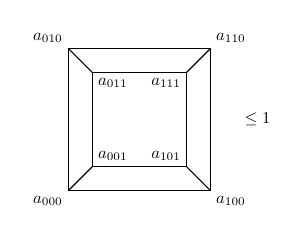
\begin{tikzpicture}[scale = 0.6, every node/.style = {scale = 0.6}]
                    \draw (0, 0) -- (3, 0) -- (3, 3) -- (0, 3) -- cycle;
                    \draw (0.5, 0.5) -- (2.5, 0.5) -- (2.5, 2.5) -- (0.5, 2.5) -- cycle;
                    \draw (0, 0) -- (0.5, 0.5);
                    \draw (3, 0) -- (2.5, 0.5);
                    \draw (3, 3) -- (2.5, 2.5);
                    \draw (0, 3) -- (0.5, 2.5);
                    \node[below left]  at (0, 0) {$a_{000}$};
                    \node[below right] at (3, 0) {$a_{100}$};
                    \node[above right] at (3, 3) {$a_{110}$};
                    \node[above left]  at (0, 3) {$a_{010}$};

                    \node[above right] at (0.5, 0.5) {$a_{001}$};
                    \node[above left]  at (2.5, 0.5) {$a_{101}$};
                    \node[below left]  at (2.5, 2.5) {$a_{111}$};
                    \node[below right] at (0.5, 2.5) {$a_{011}$};

                    \node at (4, 1.5) {$\le 1$};
                \end{tikzpicture}
            \end{center}
        \end{itemize}
    \end{column}
\end{columns}
\end{frame}

\begin{frame}
\frametitle{The two smoothing compoments of $\dP6$}
\,\,

\begin{columns}[onlytextwidth]

    \begin{column}{0.49\textwidth}
	        We can identify one component with $\P(\mathcal T_{\P^2}) \setminus H$, where $\T_{\P^2}$ is the tangent bundle of $\P^2\mkern-4mu$.
        \[
            \begin{vmatrix}
                 y  &  x_1    &  x_2    \\
                x_4 & y + t_1 &  x_3    \\
                x_5 &  x_6    & y + t_2
            \end{vmatrix}
            \le 
            1
        \]
    \end{column}
    \pause

    \begin{column}{0.49\textwidth}
	        The second component can be identified with $(\P^1 \times \P^1 \times \P^1) \setminus H$, where $H$ is a $(1,1,1)$-divisor.

        \begin{center}
	        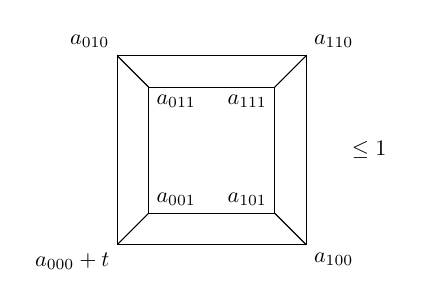
\begin{tikzpicture}[scale=0.8, every node/.style={scale=0.8}]
                \draw (0,0) -- (3,0) -- (3,3) -- (0,3) -- cycle;
                \draw (0.5,0.5) -- (2.5,0.5) -- (2.5,2.5) -- (0.5,2.5) -- cycle;
                \draw (0,0) -- (0.5,0.5);
                \draw (3,0) -- (2.5,0.5);
                \draw (3,3) -- (2.5,2.5);
                \draw (0,3) -- (0.5,2.5);
                \node[below left] at (0,0) {$a_{000} + t$};
                \node[below right] at (3,0) {$a_{100}$};
                \node[above right] at (3,3) {$a_{110}$};
                \node[above left] at (0,3) {$a_{010}$};

                \node[above right] at (0.5,0.5) {$a_{001}$};
                \node[above left] at (2.5,0.5) {$a_{101}$};
                \node[below left] at (2.5,2.5) {$a_{111}$};
                \node[below right] at (0.5,2.5) {$a_{011}$};

                \node at (4, 1.5) {$\leq 1$};
            \end{tikzpicture}
        \end{center}
    \end{column}
\end{columns}
\end{frame}
\begin{frame}
\frametitle{The two smoothing compoments}

TODO: trengs denne?


\end{frame}

\section{Mirror construction}
\begin{frame}
\frametitle{Construction of a new \CY: $X_1$}

\begin{itemize}
	\item Let $E$ be a vector space with basis $e_1,e_2,e_3$. Consider
	$$
	\P^{17} = \P(E \otimes E \oplus E \otimes E).
	$$
	The elements are pairs of $3 \times 3$ matrices, equal up to scalar multiplication.
	\item Consider the set of pairs $M$ of matrices $(A,B)$ with rank $1+1$. 
	\item Intersect $M$ with a generic $\P^{11} \subset \P^{17}$. Let $X_1 \stackrel \Delta = M \cap \P^{11}$.
\end{itemize}

\begin{theorem}
$X_1$ is a smooth \CY with Euler-characteristic $-72$.
\end{theorem}

\end{frame}


\begin{frame}
\frametitle{Construction of a new \CY: $X_2$}

\begin{itemize}
	\item Let $F$ be a vector space with basis $f_1,f_2$. Consider
	\[
        \P^{15} = \P(F \otimes F \otimes F \oplus F \otimes F \otimes),
        \alert{????}
	\]
	The elements are pairs of $2 \times 2 \times 2$-tensors, equal up to scalar multiplication.
	\item Consider the set of pairs $N$ of tensors $(A,B)$ with rank $1+1$.
	\item Intersect $N$ with a generic $\P^{11} \subset \P^{15}$. Let $X_2 \stackrel \Delta = N \cap \P^{11}$.
\end{itemize}

\begin{theorem}
$X_2$ is a smooth \CY with Euler-characteristic $-48$.
\end{theorem}

\end{frame}

\begin{frame}
\frametitle{Construction of a new \CY: $X_3$}

\begin{itemize}
	\item Let $E$ and $F$ be as before. Consider
	$$
\P^{16} = \P(E \otimes E \oplus F \otimes F \otimes).
	$$
	\item Consider the set of pairs $W$ of tensors $(A,B)$ with rank $1+1$.
	\item Intersect $W$ with a generic $\P^{11} \subset \P^{16}$. Let $X_3 \stackrel \Delta =  W \cap \P^{11}$.
\end{itemize}

\begin{theorem}
$X_3$ is a smooth \CY with Euler-characteristic $-60$.
\end{theorem}

\end{frame}

\begin{frame}
\frametitle{Hodge number heuristics}
\begin{conjecture}
$X_1$ have Hodge numbers $h^{11}=3$ and $h^{12}=39$.
\end{conjecture}
\begin{proof}[``Reason'']

\begin{enumerate}[<+->]
	\item We know the Euler characteristic, so it is enough to find $h^{12}$ ($=$ number of parameters).
	\item The Grassmannian of $\P^{11}$'s in $\P^{17}$ is $72$-dimensional.
	\item We can act by automorphism from $\prod_{i=1}^4 \GL(E)$.
	\item The subgroup $\{ t_1t_2=t_3t_4 \} \subset (\C^\ast)^4 \subset \prod_{i=1}^4 \GL(E)$ acts trivially.
	\item Hence $h^{12}=72-(\dim \prod_{i=1}^4 \GL(E) - 3) = 72-33=39$.\qedhere
\end{enumerate}

\end{proof}


\end{frame}
\begin{frame}
\frametitle{Mirror candidates}

Using the mirror Ansatz, we propose mirror candidates for $X_1$ and $X_2$.

\begin{itemize}
	\item
	BB
\end{itemize}


\end{frame}

\end{document}